\documentclass{homework}
\usepackage{ dsfont }
\usepackage{ mathtools }
\usepackage{ commath }
\usepackage[final]{ pdfpages }

\name{Timothy Devon Morris}
\course{EC En 671}
\term{Fall 2018}
\hwnum{3}

\begin{document}

\begin{problem}
  Let $A$ be a matrix that can be factored as
  \[ A = U\Sigma V^H\]
  such that
  \[ U^H U = I \quad V^HV = I\]
  and $\Sigma$ is a diagonal matrix of real values. Show that $P_A = P_U$.
\end{problem}

\begin{solution}
  The proof is pretty straight forward using the definition of the projection matrix
  \[ P_A = A(A^HA)^{-1}A^H = U\Sigma V^H(V\Sigma U^HU\Sigma V^H)^{-1}V\Sigma U^H = U\Sigma V^H(V\Sigma^2 V^H)^{-1}V\Sigma U^H \]
  Now, we need to know what the inverse of $V\Sigma^2 V^{H}$. It is $V\Sigma^{-2}V^{H}$ since
  \[ V\Sigma^2 V^{H} V\Sigma^{-2}V^{H} = I \quad \text{and} \quad V\Sigma^{-2}V^H V \Sigma^2 V^{H} = I\]
  We also note that $\Sigma^{-2}$ must exist since it is diagonal with real values. Thus we have
  \[P_A = UU^H = UIU^H = UI^{-1}U^H = U(U^HU)^{-1}U = P_U\]
\end{solution}

\begin{problem}
  Let $P_1, P_2, \dots, P_m$ be a set of orthogonal projections with $P_iP_j = 0$ for $i \neq j$. Show that $Q = P_1 + P_2 + \dots + P_m$ is an orthogonal projection. 
\end{problem}

\begin{solution}
  We first note that since $Q$ is the sum of orthogonal projections, it must be symmetric. Now let us consider $Q^2$, we note that all the mixed terms will disappear.
  \[ Q^2 = P_1^2 + P_2^2 + \dots + P_m^2 =  P_1 + P_2 + \dots + P_m = Q\]
  Thus, $Q$ is a orthogonal projection.
\end{solution}

\begin{problem}
  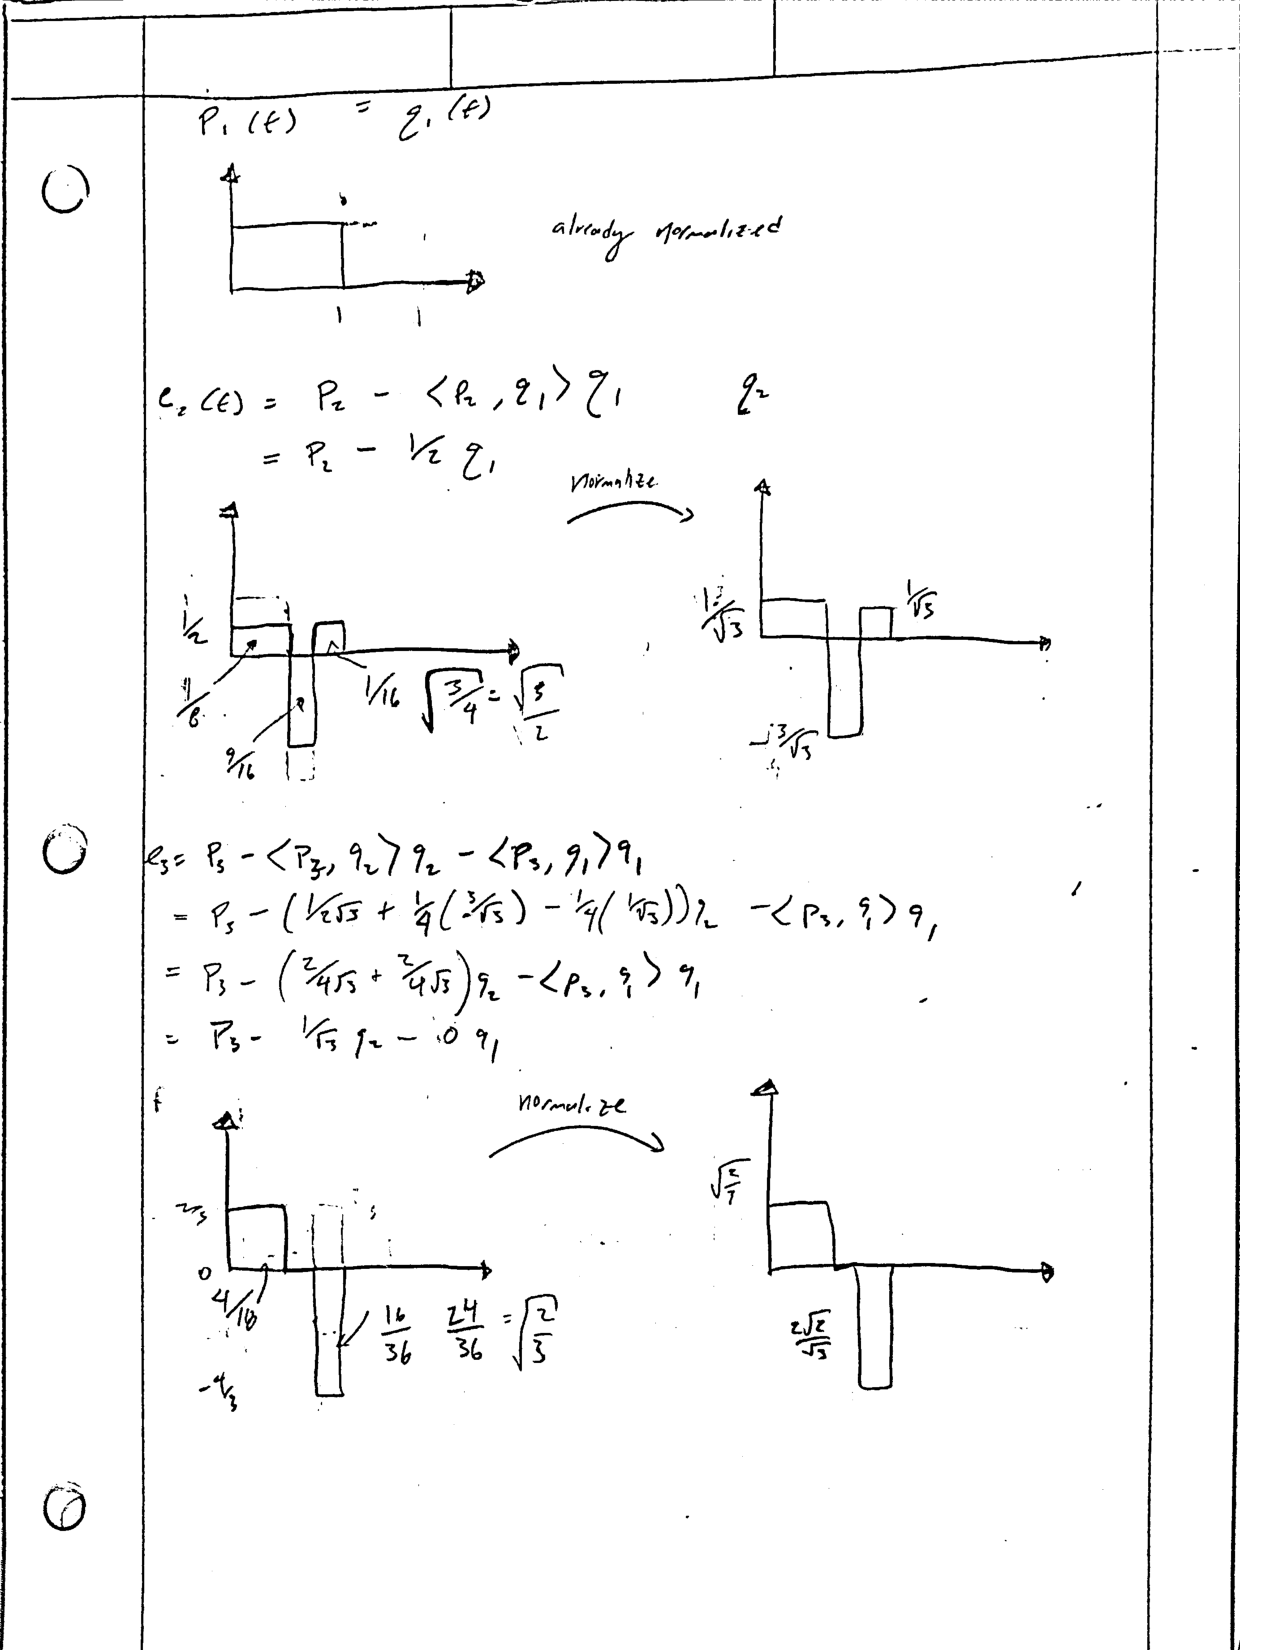
\includepdf[pages=-]{hw3prob3.pdf}
\end{problem}

\begin{problem}
\end{problem}

\end{document}
